\documentclass[letter, 11pt]{article}
\usepackage[utf8]{inputenc}
\usepackage[spanish]{babel}
\usepackage{amsfonts}
\usepackage{amsmath}
\usepackage[dvips]{graphicx}
\usepackage{url}
\usepackage{hyperref}
\usepackage[top=3cm,bottom=3cm,left=3.5cm,right=3.5cm,footskip=1.5cm,headheight=1.5cm,headsep=.5cm,textheight=3cm]{geometry}
\usepackage{listings}
\usepackage{color}
\usepackage{fancyvrb}
\usepackage{fancyhdr}
\usepackage{setspace}
\renewcommand{\rmdefault}{phv} % Arial
\renewcommand{\sfdefault}{phv} % Arial

\definecolor{red}{rgb}{1,0,0}
\definecolor{green}{rgb}{0,1,0}
\definecolor{blue}{rgb}{0,0,1}
\newcommand{\blue}{\textcolor{blue}}
\newcommand{\red}{\textcolor{red}}
\newcommand{\green}{\textcolor{green}}


%%%%%%%%%%%%%%%%%%%%%%
%Estilo del documento%
%%%%%%%%%%%%%%%%%%%%%%
\pagestyle{fancy}
\onehalfspacing

%%%%%%%%%%%%%%%%%%%%%%%%%%%%%%%%%%%%%%%%%%%
%Fancyheadings. Top y Bottom del documento%
%%%%%%%%%%%%%%%%%%%%%%%%%%%%%%%%%%%%%%%%%%%
% Recuerde que en este documento la portada del documento no posee
% numeracion, pero de igual manera llamaremos a esa primera pagina la numero
% 1, y la que viene la dos. Esto es para tener una idea de las que
% llamaremos pares e impares
\lhead{Evaluación de Proyectos - Primer Informe} %Parte superior i\include{quierda}
%\rhead{\bf \it Primer Informe} %Parte superior derecha
\lfoot{Universidad Técnica Federico Santa María} %Parte inferior i\include{quierda.}
\cfoot{} %Parte inferior central
\rfoot{\bf \thepage} %Parte inferior derecha
\renewcommand{\footrulewidth}{0.4pt} %Linea de separacion inferior

\begin{document}
\renewcommand{\tablename}{Tabla}

\renewcommand{\listtablename}{Índice de tablas}

\begin{titlepage}
    \begin{center}
	\begin{tabular}{c}
		
\includegraphics[width=0.4\textwidth]{img/utfsm}
	    \vspace{4cm}
	\end{tabular}
	\vspace{6cm}
	\begin{tabular}{c}
		\huge{\sc{Trabajo Recuperativo}}\\\\
		\large{\sc{Evaluación de Proyectos}}
	\end{tabular}
    \vspace{1cm}
	\begin{tabular}{rcl}
			Nombre del Profesor & : & Johana Moya Alfaro\\
			Nombre del Ayudante & : & Teresa Paez\\
								& : & Melissa Ruiz\\
			Datos del Alumno    & : & Cristián Maureira\\
                                & : & 2673030-9
	\end{tabular}

    \vspace{1cm}

    \normalsize{\sc{\today}}\\

	\end{center}
\end{titlepage}


\tableofcontents
\listoffigures
\listoftables


\section{Introducción}

\section{Resumen Ejecutivo}
Mediante el presente proyecto presentado por \textsc{Music Labs}
se evaluará la creación de un centro multidisciplinario que integre los
distintos procesos por los cuales debe pasar una banda emergente alcanzar el éxito.

% En primera instancia el servicio será ofrecido en la V región, para luego evaluar
%la posibilidad de expansión en la distintas regiones de Chile.

\textsc{Music Labs} será un servicio que reunirá todos los elementos para lanzar
una banda musical emergente a la fama. Entre estos elementos se encuentran:
estudio de grabación, sala de ensayo, salón de eventos, asesoría personal 
y posicionamiento en la Web 2.0. Esto se justifica en el hecho que actualmente
en Chile no existe un servicio que integre todos estos procesos en un solo servicio.

El estudio de mercado muestra que existe un aumento en la cantidad de 
bandas emergentes en la V región, esto motivado principalmente por dos factores a destacar:
La disminución de los valores de instrumentos y la masificación de los medios de 
comunicación como Internet. Además el estudio muestra que el segmento
objetivo se compone de la población adulto-joven, específicamente personas mayores 
de 18 años pertenecientes a los grupos socioeconómicos C2 y C3 los cuales representan 
el $55\%$ del mercado de la V región.

El análisis de la oferta indica que los principales competidores son salas de 
ensayo tradicionales y estudios de grabación. Generalmente estos servicios se 
ofrecen por separado. El $92\%$ de las salas de ensayo se concentra en la región
Metropolitana, de las restantes sólo el $4\%$ se encuentra en la V región.
Con respecto a los estudios de grabación el $85.2\%$ se encuentra en la R.M, mientras
que sólo un $5.8\%$ se encuentra en la V región.

 Por lo tanto, \textsc{Music Labs} se presenta como un proyecto innovador 
que posee una gran ventaja competitiva por ser un servicio
orientado al cliente apoyado por un equipo de profesionales altamente capacitados.


\section{Conclusiones}

\textsc{Music Labs} dará oportunidades a muchas
bandas de la región, provocando un cambio radical
durante la etapa de maduración de las bandas emergentes.
La idea planteada está ligada a fomentar el desarrollo cultural
en la región, explotando un nicho que hasta el momento
sólo había sido atacado por sectores, ya que no existe
una oferta clara en este ambiente. Este desarrollo
también irá ligado directamente con nuevas
posibilidades de trabajo para músicos de la zona a través
de las distintas oportunidades que surgen a raíz
del trabajo que van realizando a medida que se
hacen más conocidos.


Hoy en día es más común ver nuevas bandas musicales gracias al mayor acceso a internet y a la disminución
de los precios de los instrumentos y equipos musicales.

No hay un registro histórico de las bandas que han ido surgiendo en nuestro país, por ende es muy difícil
recabar datos para hacer un análisis de demanda. Sin embargo se buscó por internet y se hizo una proyección
de demanda que arroja una tendencia  al crecimiento en la cantidad de bandas que se van formando año a año.

Según datos entregados por el club de música, nuestra universidad tiene 23 bandas, asumiendo que la cantidad de bandas es
proporcional a la cantidad de alumnos se estimó un total de 143 bandas en las universidades pertenecientes al consejo de rectores de
la región. Existen sólo 7 locales importantes que ofrecen servicios de sala de ensayo y/o estudio de grabación en la V región.

Se consultó a músicos de la zona y se concluyó que una banda en promedio trabaja 4 horas semanales en una sala de ensayo.

 
La V región tiene características deseables para llevar a cabo el proyecto, como por ejemplo tener una
gran cantidad de estudiantes y de personas pertenecientes al nivel socioeconómico C2 y C3. 



Se ha realizado un primer análisis con respecto a varios
aspectos del proyecto, que lo deja mejor
posicionado para enfrentar los retos que irán apareciendo en
el camino.

Debido al claro crecimiento de las bandas emergentes
tanto en la región como el país, es evidente
el nivel de importancia que tiene la evolución musical que se viene 
gestando desde algunos años en Chile.

A través de los servicios que \textsc{Music Labs} ofrece,
se está haciendo un llamado de atención
a las diferentes fuentes de apoyo a la música nacional
para dar a conocer el potencial artístico que tiene la zona.

Se ha generado además un estudio inicial con respecto
a las situaciones relacionadas con el proyecto,
sin dejar de lado un análisis fundamental que era ver
la separabilidad del proyecto, lo que impulsó
la idea de tener un servicio principal
compuesto de otros servicios más particulares.

Por otro lado fue importante listar y describir
los principales elementos para dimensionar los costos
y beneficios que poseía el proyecto. 

El hecho de realizar un análisis de la demanda y oferta, ilustra
el comportamiento de las bandas en constante crecimiento, por lo que
satisfacer las necesidades de manera íntegra es una oportunidad valiosa.

\section{Diagnóstico}

\subsection{Definición de la Idea del Proyecto}
La idea general que desarrolla este proyecto está centrada en la necesidad 
actual de la gran mayoría de las bandas musicales emergentes. Una agrupación 
musical requiere un lugar que le brinde el soporte técnico necesario 
para componer y ensayar su música. En una etapa previa la banda 
requiere grabar sus composiciones para dejar registro y poder hacer 
conocido públicamente su trabajo. \\

Lamentablemente, muchas bandas se quedan estancadas en esta etapa, ya 
que no tienen posibilidades concretas de mostrar su trabajo al 
público. Un público que si bien existe, no tiene la oportunidad de 
conocer nuevas bandas por las pocas opciones de difusión con que 
cuentan las bandas emergentes.\\

Este proyecto está enfocado en crear una instancia que permita a las 
bandas nuevas, componer, grabar y difundir su trabajo musical. 

\subsection{Objetivos del proyecto}
	%\subsubsection{Objetivo General}
	Entregar un servicio diferenciado y multidisciplinario 
	que integre los distintos procesos por los cuales 
	debe pasar una banda musical emergente al momento 
	de lanzar su carrera. 
	
	Posicionar a \emph{Music Labs} como el mejor
	proveedor de este servicio en la región, siendo una incubadora
	de bandas emergentes que demuestre
	entregar además de los espacios físicos,
	la asesoría necesaria para dar soporte a las distintas demandas de las 
	bandas musicales actuales.

	Utilizar los medios electrónicos actuales
	para dar a conocer a las distintas bandas
	emergentes que utilicen el servicio,
	a nivel regional, nacional y mundial

	
	
	%Además, entregar asesorías en cada uno de estos 
	%procesos a través de profesionales capaces de 
	%guiar y evaluar el trabajo realizado por las 
	%distintas bandas cubriendo las distintas necesidades 
	%de ellas.

	%\subsubsection{Objetivos Específicos}
	%Crear un completo servicio de apoyo al lanzamiento de una 
	%banda musical que cuente con lo siguiente:
	%	\begin{itemize}
	%		\item Sala de ensayo con los implementos 
	%			necesarios que permita a una banda musical 
	%			desarrollarse profesionalmente.
	%		\item Estudio de grabación que cuente con la presencia 
	%			de profesionales expertos en grabación y producción 
	%		\item Salón de eventos, para poder crear una primera instancia
	%			de un espectáculo abierto al público de las nuevas bandas.
	%		\item Productora de eventos, cuya misión será la organización 
	%			y difusión de encuentros entre las distintas bandas.
	%		\item Managers a la disposición de las bandas que lo requieran.
	%		\item Difusión de las bandas a través de Internet lo cual 
	%			contempla la creación de una página Web por cada banda 
	%			y el posicionamiento de esta en las redes sociales 
	%			más populares como Facebook y Twitter.
	%	\end{itemize}

\subsection{Antecedentes generales del proyecto}

El mayor problema que enfrenta una agrupación o banda musical al momento
de comenzar una carrera es encontrar la asesoría adecuada para iniciar
una carrera rentable en este mercado competitivo. La primera dificultad
es encontrar una adecuada sala de ensayo que cuente con todos los 
implementos necesarios para que las bandas mejoren su calidad musical. 
Una vez encontrada una buena sala de ensayo, algunas bandas deciden grabar
su primer disco y entrar en el mercado. Las bandas de regiones se encuentran
con el hecho de que los mejores estudios de grabación se encuentran en Santiago.

Por otra parte, la difusión de la banda en muchos casos es responsabilidad
de los mismos integrantes. Entre estas tareas se encuentra buscar y utilizar
los medios para poder difundir su música.

Concretamente, existen pocos eventos donde se dé el espacio a una banda 
emergente de presentar su música para ser conocidos a nivel nacional
o internacional. Este punto es un riesgo que asume la banda al lanzar
su carrera.

Es por esto que actualmente en Chile existe una necesidad para las bandas 
emergentes de contar con un servicio integral que cuente con los implementos
necesarios que permitan que las bandas ensayen sus canciones, graben sus discos
y finalmente difundan su trabajo para entrar en el competitivo mercado
de la música. La distribución de estos recursos es totalmente centralizada. En 
Chile existe un total de 175 salas de ensayo, de las cuales un 92\% de ellas 
se encuentran en la ciudad de Santiago, mientras que el porcentaje
restante se distribuye a lo largo del resto del país.

Con respecto a los estudios de grabación, la distribución es similar, con un
84,6\% de ellos ubicados en Santiago y el resto en regiones. 

En cuanto al apoyo en difusión y eventos, ninguno de estos servicios antes 
mencionados cuenta con un apoyo integral a las bandas.

\subsection{Alcance del proyecto}

El proyecto se realizará en primera instancia 
en la V región y estará enfocado a bandas emergentes 
que necesiten soporte musical para ensayar y 
componer su trabajo. Además obtendrán apoyo 
en difusión mediante eventos organizados 
especialmente para apoyar el inicio de todas 
las bandas que utilicen el servicio.\\

Con respecto a los eventos, estos se realizarán en 
un comienzo en la región mediante convenios 
con locales asociados al proyecto y en un centro de eventos
propio  del servicio ubicado en la V Región. La frecuencia 
de estos están sujetos a la cantidad de locales 
asociados y su disponibilidad.\\

La difusión se realizará en 
las distintas redes sociales más populares del 
momento y su éxito será medido de acuerdo a 
la cantidad de personas que visiten la información 
de la banda.\\

Con respecto al servicio, la banda musical 
que acceda al servicio, contará con los implementos 
necesarios para realizar sus ensayos, grabar sus 
discos, actuar en eventos regionales o nacionales 
y el respaldo tecnológico para su difusión en 
el mundo a través de Internet, para así alcanzar 
el éxito.\\

La cantidad de Managers disponibles dependerá de los
contactos que maneje el proyecto y las bandas podrán 
solicitar la información de contacto de estos.\\

Cabe destacar que, si bien, algunos estudios 
de grabación incluyen sala de ensayo, ninguno 
de ellos ofrece un servicio completo de 
difusión y asesoría para las bandas musicales 
lo cual hace que el proyecto planteado tenga 
una ventaja competitiva, ya que está 
orientado al cliente en todo aspecto.

\subsection{Justificación del proyecto}

Del 100\% de salas de ensayo que se encuentran en el país (172), el 92\% 
se concentra en la región metropolitana. De las restantes, sólo 7 salas se 
encuentran en la V región (correspondiente al 4\%). Si se utilizan los
datos demográficos obtenidos desde los resultados del censo realizado 
en el año 2002 en Chile, se puede observar que, si bien el 40\% de la 
población total del país se concentra en la región metropolitana, más
del 20\% se encuentra repartido entre la V y la VIII región. Esto indica que, 
de existir una relación equitativa entre las salas de ensayo y estudios de
grabación, y la población total, al menos el 20\% del total de salas de 
éstas deberían existir entre estas regiones. Pero, ¿Por qué realizar 
esta comparación ? La razón es muy simple. Las personas que tienden a 
formar grupos de música, realizar tocatas, etc, son el público adolescente
 - adulto joven. Esto incluye mayormente a los estudiantes de educación media
y universitarios (personas entre 15 y 30 años mayormente). La zona de la V 
región es conocida por la cantidad de estudiantes que posee. De hecho, 
se puede encontrar 4 universidades pertenecientes al consejo de rectores, de
gran prestigio (lo que implica que gran cantidad de estudiantes se acercará
a estas instituciones), además de una serie de universidades privadas 
líderes en cada uno de sus ámbitos, y una serie de Institutos de Educación
superior y Centros de Formación Técnica. Por lo tanto, existe una alta
presencia de personas a las cuales ofrecer el nuevo servicio que se propone.

\subsection{Impacto del proyecto}

Chile posee una gran diversidad musical y 
cultural que perdura en el tiempo mediante la 
composición nueva música y la reversión de 
temas que ya son parte del mundo cultural 
de Chile. Este proyecto permitirá aumentar 
el abanico de bandas y solistas que trabajan 
en el mundo de la música y que no tienen 
las mismas oportunidades de difusión que 
las grandes bandas. Esto, a través de un 
servicio de calidad y costo apropiado según 
la realidad de las nuevas bandas. Además, al
contar con mayor diversidad de bandas es posible
aportar a la difusión cultural de la música
del país, ayudando a que la generación actual
y futura conozca la música que se hizo y que
se está haciendo a nivel local y nacional.\\ %(IMPACTO CULTURAL)

En la actualidad, el precio de los instrumentos 
musicales ha disminuido considerablemente respecto 
a décadas anteriores. Esto ha permitido que muchas 
personas tengan la oportunidad de adquirir instrumentos 
y tener como hobbie la ejecución musical. Es por esto 
que la cantidad de bandas emergentes también aumentó 
con el paso del tiempo. Este proyecto permite a las 
nuevas bandas ir un paso más adelante, dejando de 
tener una banda como pasatiempo y pasar a ser 
una banda profesional. Así. la idea acá presentada 
tendrá gran impacto social, al ser una nueva 
fuente de trabajo y desarrollo social y cultural 
para muchas personas.\\ %(IMPACTO SOCIAL)

Es posible visualizar un impacto negativo %IMPACTO ACÚSTICO A LOS VECINOS.
relacionado con la contaminación acústica
generada por alto nivel de sonido que emanará
del salón de eventos. El salón, al estar
ubicado en un sector céntrico de la ciudad
es posible que cause molestia a las personas
que vivan en los alrededores, no solo debido
al sonido sino también a los efectos producidos
por la gente que asiste a los eventos.\\

A nivel local, el proyecto tendrá cierto impacto
en el nivel de empleabilidad de la región, ya que
para la implementación será necesario contar con
distintos profesionales encargados de las distintas
áreas abarcadas por \emph{Music Labs}. Hay que destacar
que no será un impacto mayor por no ser necesario una
alta cantidad de trabajadores, pero si se convierte
en una fuente de trabajo para la región.

\section{Metodología}

\subsection{Identificación de la Situación actual}

% Pocas entidades que brinden todos estos servicios.

Actualmente en la región de Valparaíso existen diversos servicios enfocados a
bandas de música, pero ninguno de ellos ofrece el servicio completo consistente en salas de
grabación, salas de ensayo, promoción/difusión, traslado a eventos, etc.

Además, la región se caracteriza por su alta oferta de actividades recreativas,
enfocándose en gran parte al área turística y recreacional a lo largo de todo el año.

Dentro de éste contexto, existen a su vez un sinnúmero de bares y pubes en los que
múltiples bandas ofrecen sus servicios gratuitamente en búsqueda de promoción
propia, para lograr ser más conocidas y aumentar sus posibilidades de trabajo.

Si las bandas no tuvieran que
gastar tanto esfuerzo en la promoción y búsqueda de eventos en los que estar
presentes, podrían dedicar más tiempo a la creación musical, y generando
alianzas estratégicas con los diferentes locales de recreación se puede generar
una mayor difusión de las bandas que presenten en cada uno de ellos.

\subsection{Situación Base}

% Corresponde a la situación actual optimizada.
% ¿Qué pasa si no se realiza el proyecto?
% La optimización de la situación actual es a nivel de gestión y de eficiencia,
%  implica la realización de inversiones significativas.

El proyecto se iniciará desde cero,
y por el momento no existen alternativas que sean equivalentes al servicio completo
que se ofrecerá.

Las únicas aproximaciones podrían ser los centros que hoy en día
tienen a lo más sala de ensayo y grabación, pero no son comparables
debido a que aquellas características sólo son una parte de la idea propuesta.

\subsection{Situación con proyecto}

% Se proyecta como sería el escenario realizando el proyecto.
% Se analizan todos los impactos, positivos o negativos, que generará la realización
%  del proyecto.

Tomando en cuenta la situación actual para todos los grupos musicales
que nacen en Chile se estaría provocando un cambio radical en la mentalidad
de las bandas emergentes, pues se estaría creando un proyecto
nunca antes visto, el cual fomentaría la experiencia musical en Chile.

Al ofrecer un conjunto de servicios relacionados y con el mismo objetivo,
lograr que una banda se posicione como una banda famosa a nivel nacional,
es difícil que cualquier banda emergente rechace la oferta.

Pero, además de fomentar la madurez musical de las nuevas bandas
de Chile, se está potenciando la música en chile,
lo que puede provocar a largo plazo un cambio de mentalidad
en la población chilena, para poder considerar aún más
lo que vendría siendo el producto nacional.

\subsection{Comparación situación base y situación con proyecto}

Actualmente no existe oferta alguna del servicio propuesto, por lo que el
público objetivo debe encargarse de gran parte de la difusión y promoción.

\subsection{Separabilidad de Proyectos}

% Las unidades estratégicas son aquellas que no se pueden separar.
% Dividir el proyecto en dos o más subproyectos.
% Los proyectos son separables en la medida que se pueda identificar un producto
%  o servicio a transferir y un precio de transferencia.
%
% Explicar que para simplificar el proyecto no se planeará dividir el proyecto
%  en diferentes empresas o cosas por el estilo.
% Nuestro proyecto puede llevarse a cabo a través de una sola empresa que preste
%  todos los servicios anteriormente mencionados, esto porque justamente uno los
%  objetivos es ofrecer el servicio completo a nuestros clientes, evitando que
%  deban recurrir a diferentes instancias y abaratando costos (Juan).

Debido a las características del presente proyecto
se puede fácilmente notar que es perfectamente separable
en varias unidades estratégicas, como:

\begin{itemize}
	\item Salas de ensayo.
	\item Estudios de grabación.
	\item Posicionamiento en redes sociales y web 2.0.
	\item Salas de eventos.
\end{itemize}

Si bien es cierto,
cada uno de los puntos anteriormente señalados puede
verse como un producto final que será adquirido
por los potenciales clientes a un determinado
valor, no va de la mano con nuestra propuesta.

A lo largo de Chile existen distintas
empresas que brindan algunos de estos servicios,
pero ninguna ha realizado la labor de poder
ofrecer un producto más generalizado y completo,
es por eso que no se planea dividir el proyecto,
pues se estaría poniendo a disposición de terceros
alguno de los servicios que serían los pilares fundamentales
de nuestra propuesta, ya que se pretende provocar
la confianza de los clientes, al poder recurrir
a nosotros y brindarles un servicio completo
de primera calidad, evitando tener que buscar
en diferentes lugares, a veces en distintas regiones
de Chile, intentando conseguir  una cierta
cantidad concreta de elementos vitales
para lo que es la evolución de una \emph{``Banda Musical''}.

\subsection{Métodos de medición de beneficios y costos }

% Obedece a procedimientos establecidos de valoración.
% Definición de la forma de evaluación de los movimientos de fondos.
%  (permiten construir un flujo de caja)
% Identificación de los costos de inversión, operaciones,
%  beneficios directos e indirectos.
%
% El procedimiento general consiste en la identificación de las variables,
%  ya sean de beneficios y costos; luego la cuantificación de ellas en unidades
%  física, siempre y cuando las variables sean factibles de cuantificar; y 
%  posteriormente se procede a la valoración monetaria, es decir, asignarle
%  un precio o costo a ellas.

\subsubsection{Inversión}
\begin{itemize}
	\item Arriendo de local:
			Se necesita un local ubicado en lo ideal en el sector céntrico de Viña del Mar,
			con suficiente espacio para dos salas de ensayo, una sala de grabación, una oficina
			y un salón de eventos.
			Cada sala de ensayo debe ser de al menos 12 metros cuadrados,
			la sala de grabación y la oficina de al menos 9 metros cuadrados cada una,
			el salón de eventos podría estar ubicado perfectamente en otro lugar,
			o en el mismo establecimiento, para favorecer la llegada de público.
	\item Equipos:
			Se necesitarán amplificadores, altavoces, mesas, reproductores, entre otros.
	\item Instrumentos:
			Se necesitarán diversos instrumentos entre los cuales destacan guitarras, bajos, baterías,
			teclados, micrófonos, entre otros.
	\item Publicidad:
			Este punto será el más importante, pues se necesita llegar a todos los rincones posibles,
			por lo que la inversión en publicidad es esencial.
			Se requerirán anuncios publicitarios en radios, internet, afiches en centros de eventos,
			pubes, etc, teniendo como principal misión, comunicar el proyecto en lugares
			frecuentados por músicos.
\end{itemize}

\subsubsection{Ingresos}
\begin{itemize}
	\item Arriendo Sala Ensayo:
			Se obtendrán ingresos por el concepto de arriendo por hora de la sala de ensayos.
	\item Contratación grabación disco:
			Se prestará el servicio de grabación y asesoría técnica para la grabación de un
			disco con los temas seleccionados por la banda.
			El valor dependerá de la duración del disco y de la complejidad del equipo
			e instrumentos necesarios para su grabación.
	\item Contratación posicionamiento web:
			Se prestarán servicios de publicidad para bandas que deseen difusión a través
			de internet, haciendo uso de redes sociales y en caso de que la banda no posea
			sitio web, también puede pagar por la creación y mantención de uno.
	\item Traslados:
			Se ofrecerá el servicio de traslado de bandas a distintos eventos en la zona.
	\item Contratación sistema completo:
			Se ofrecerán todos los servicios anteriores por un precio mucho más conveniente
			para los clientes, sin duda una de las características diferenciadoras de
			nuestra empresa con respecto a lo que se ofrece en el mercado.
\end{itemize}

\subsubsection{Costos fijos}
\begin{itemize}
	\item Salarios:
			Costo fijo mensual para pago de empleados de la empresa entres los cuales se cuentan:
			técnicos en sonido, secretaria y ayudantes.
	\item Servicios básicos:
			Costo de agua,luz y otros inherentes a la mantención del local.
	\item Servicios adicionales:
			Costo de servicios adicionales como teléfono e internet.
	\item Seguros:
			Seguros de robo e incendio.
	\item Mantención:
			Costo fijo mensual de mantención de aseo, reparación de equipos, entre otros.
\end{itemize}


\subsection{Método de evaluación de rentabilidad que se usará}

Es posible encontrar variados
métodos para valorizar las inversiones, 
los cuales se pueden agrupar en dos grandes categorías: los métodos \emph{dinámicos} y los métodos \emph{estáticos}.

Los \emph{métodos estáticos} no consideran
el tiempo como un factor importante,
es decir, que no se considerará el momento en el cual
pueda existir una salida o entrada de dinero al
proyecto.

Algunos ejemplos de \emph{métodos estáticos} son:
\begin{itemize}
	\item El método del Pay-Back o Plazo de recuperación.
	\item El método del flujo neto de caja (Cash-Flow estático).
	\item El método de la Tasa de rendimiento contable.
\end{itemize}

Por otro lado,
los \emph{métodos dinámicos}, van a suplir el problema
que poseen los métodos estáticos, ya que si van a tomar
en consideración el tiempo en que se producen entradas
o salidas de dinero.

Algunos ejemplos de \emph{métodos dinámicos} son:
\begin{itemize}
	\item La Tasa de Rentabilidad Interna (T.I.R).
	\item La Tasa de Rentabilidad Interna Modificada(T.I.R.M).
	\item El Valor Actual Neto (V.A.N).
	\item El Pay-Back dinámico (o descontado).
\end{itemize}

El problema que se podría considerar es que éstos métodos
nos entregan información de una cierta porción del
proyecto, por lo cual es muy recomendado poder utilizar
el complemento de éstos tres métodos, para poder
tener una visión mucho más completa de la situación
actual del proyecto.

Es por la razón anterior, que el proyecto utilizará
los métodos dinámicos nombrados anteriormente.

\subsubsection{Tasa Interna de Rentabilidad}

Cuando se habla de Tasa Interna de Rentabilidad (T.I.R.)
se refiere a una tasa de descuento que produce que el Valor Actual Neto (V.A.N),
de una inversión igual a cero.

Pero, ¿De qué nos sirve éste método?

Si la T.I.R. que resulte va a superior o igual a la tasa exigida por el inversor,
tomando en consideración variadas alternativas, la que nos entregue
una T.I.R. mayor, será más conveniente.

Pero, ¿Qué tan complejo es su cálculo?

Éste método es conocido por ser muy difícil de calcular (método iterativo),
pero hay variadas alternativas que nos ayudarán a tener un trabajo más fácil, ya sean utilizando
planillas de cálculo, técnicas matemáticas como la interpolación lineal, o calculadoras
especializadas.

%	Pero la más importante crítica del método (y principal defecto) es la inconsistencia
%	matemática de la T.I.R. cuando en un proyecto de inversión hay que efectuar otros
%	desembolsos, además de la inversión inicial, durante la vida útil del mismo, ya sea debido a
%	pérdidas del proyecto, o a nuevas inversiones adicionales.
%	La T.I.R. es un indicador de rentabilidad relativa del proyecto, por lo cual cuando se hace
%	una comparación de tasas de rentabilidad interna de dos proyectos no tiene en cuenta la
%	posible diferencia en las dimensiones de los mismos. Una gran inversión con una T.I.R.
%	baja puede tener un V.A.N. superior a un proyecto con una inversión pequeña con una
%	T.I.R. elevada.

\subsubsection{Tasa Interna de Rentabilidad Modificada}
	Esta tasa fue diseñada con la finalidad de superar las deficiencias de la T.I.R. 
	La tasa T.I.R.M tiene en consideración la posibilidad de reinvertir los flujos incrementales de fondos del proyecto a una tasa equivalente al costo de capital de la empresa, a diferencia de la T.I.R que supone la reinversión de los flujos a la tasa interna de retorno del proyecto.
	Esta tasa también se conoce como tasa de retorno o recuperación externa.

\subsubsection{Valor Actual Neto}

Se entiende como Valor Actual Neto (V.A.N) de una determinada inversión realizada,
como la sumatoria de todos los valores actualizados, considerando todos los flujos
de caja esperados (netos), los cuales se pueden deducir del valor inicial
que se utilizó cuando se comenzó la inversión, lo cual claramente es una ventaja.

Las características fundamentales para que un proyecto sea rentable son:
\begin{itemize}
	\item Se considera un proyecto $A$ y un proyecto $B$, se calcula los V.A.N.
		  de cada uno, $vanA$ y $vanB$, el que posea un V.A.N. más alto
		  será el proyecto más rentable.
	\item Si el V.A.N. posee un valor positivo, es rentable, en cambio
		  si su valor es nulo, se sabrá que la rentabilidad será equivalente
		  a disponer los fondos en un mercado determinado, considerando un cierto
		  interés equivalente a la tasa de descuento que se ha utilizado.
\end{itemize}

Debido a que el presente proyecto será financiado en su totalidad mediante un préstamo,
se fijará el valor de la tasa de interés, se utilizará el costo de la deuda.


%	Conocido bajo distintos nombres, es uno de los métodos más aceptados (por no decir el que
%	más).
%	Por Valor Actual Neto de una inversión se entiende la suma de los valores actualizados de
%	todos los flujos netos de caja esperados del proyecto, deducido el valor de la inversión
%	inicial.
%	Si un proyecto de inversión tiene un VAN positivo, el proyecto es rentable. Entre dos o más
%	proyectos, el más rentable es el que tenga un VAN más alto. Un VAN nulo significa que la
%	rentabilidad del proyecto es la misma que colocar los fondos en él invertidos en el mercado
%	con un interés equivalente a la tasa de descuento utilizada. La única dificultad para hallar el
%	VAN consiste en fijar el valor para la tasa de interés, existiendo diferentes alternativas.
%	
%	Como ejemplo de tasas de descuento (o de corte), indicamos las siguientes:
%		a) Tasa de descuento ajustada al riesgo es la suma entre Interés que se puede obtener
%		   del dinero en inversiones sin riesgo (deuda pública) y la prima de riesgo.
%		b) Coste medio ponderado del capital empleado en el proyecto.
%		c) Coste de la deuda, si el proyecto se financia en su totalidad mediante préstamo o
%		   capital ajeno.
%		d) Coste medio ponderado del capital empleado por la empresa.
%		e) Coste de oportunidad del dinero, entendiendo como tal el mejor uso alternativo,
%		   incluyendo todas sus posibles utilizaciones.
%	
%	La principal ventaja de este método es que al homogeneizar los flujos netos de Caja a un
%	mismo momento de tiempo (t=0), reduce a una unidad de medida común cantidades de
%	dinero generadas (o aportadas) en momentos de tiempo diferentes. Además, admite
%	introducir en los cálculos flujos de signo positivos y negativos (entradas y salidas) en los
%	diferentes momentos del horizonte temporal de la inversión, sin que por ello se distorsione
%	el significado del resultado final, como puede suceder con la T.I.R.
%	Dado que el V.A.N. depende muy directamente de la tasa de actualización, el punto débil
%	de este método es la tasa utilizada para descontar el dinero (siempre discutible). Sin
%	embargo, a efectos de “homogeneización”, la tasa de interés elegida hará su función
%	indistintamente de cual haya sido el criterio para fijarla.
%	
%	El V.A.N. también puede expresarse como un índice de rentabilidad, llamado Valor neto
%	actual relativo, expresado bajo la siguiente fórmula:
%		VAN relativo = VAN de la inversion / Inversion
%	O bien en forma de tasa (%):
%	
%		Tasa VAN relativo = VAN de la inversion / Inversion * 100
%
\subsubsection{Pay-Back dinámico}

El Pay-Back dinámico busca solucionar el problema principal del Pay-back estático,
el cual es que no considera los valores actuales de los flujos de caja de los últimos
periodos, por lo que un método dinámico siempre será más actualizado, pero incompleto.

El Pay-Back dinámico corresponde al periodo de tiempo necesario para poder recuperar
el capital invertido en cierto proyecto.

La idea principal es poder calcularlo para complementar el estudio de la valorización
del riesgo de una inversión determinada, en casos complejos de predecir la tasa de
depreciación de la inversión, que ocurre muy frecuentemente.

% ------------------------ lo de abajo no iría ---------------------------


% Es costumbre evaluar los proyectos mediante la aplicación de criterios convervadores
%  (VAN y TIR), no obstante en algunos proyectos será necesario emplear criterios específicos
%  como por ejemplo, para el caso de evaluación de proyectos sociales del área salud, un
%  indicador puede ser el número de pacientes senados o atendidos anualmente.
% El contenido de la metodología de evaluación varía en tamaño de 10 a 20 páginas.
%----------------
%
%
%Rentabilidad
%
%Para obtener la rentabilidad financiera del proyecto se utilizara el indicador ROE (return on
%equity), el cual relaciona el beneficio económico con los recursos necesarios para obtener ganancia.
%Luego, para demostrar porque fue ganada una cierta rentabilidad financiera se utilizara la Fórmula de
%Du Pont, la cual analiza detalladamente las causas que generaron la rentabilidad.
%
%ROE = Beneficio Neto / Patrimonio Neto
%
%Formula de Du Pont = Beneficio Neto / ventas × Patrimonio Neto / ventas
%
%Evaluación de la inversión
%	Dentro de los modelos de evaluación de inversiones evaluamos los seis métodos
%	existentes determinando el más acorde a nuestro proyecto:
%Flujo neto de caja
%	Def 1:
%	Este método comprende la suma de todos los cobros menos todos los pagos efectuados durante
%	la vida útil del proyecto de inversión. Debido a su poca utilidad practica de este método consideramos
%	descartarlo.
%
%	Def 2:
%	Por Flujo neto de Caja, se entiende la suma de todos los cobros menos todos los pagos
%	efectuados durante la vida útil del proyecto de inversión. Está considerado como el método
%	más simple de todos, y de poca utilidad práctica.
%	Existe la variante de Flujo neto de Caja por unidad monetaria comprometida, la cual es el
%	cociente entre el Flujo neto de Caja y la Inversión inicial.
%
%PayBack estático
%	Def 1:
%	Debido a que este método considera aquellos proyectos cuyos beneficios permiten recuperar
%	más rápidamente la inversión, consideramos que no es apropiado para nuestro caso por el largo plazo
%	de recuperación de la inversión.
%
%	Def 2:
%	Es el número de años que la empresa tarda en recuperar la inversión. Este método
%	selecciona aquellos proyectos cuyos beneficios permiten recuperar más rápidamente la
%	inversión, es decir, cuanto más corto sea el periodo de recuperación de la inversión mejor
%	será el proyecto.
%	Los inconvenientes que se le atribuyen, son los siguientes:
%	
%		a) El defecto de los métodos estáticos (no tienen en cuenta el valor del dinero en las
%		   distintas fechas o momentos)
%		b) Ignora el hecho de que cualquier proyecto de inversión puede tener corrientes de
%		   beneficios o pérdidas después de superado el periodo de recuperación o reembolso.
%	
%	Puesto que el plazo de recuperación no mide ni refleja todas las dimensiones que son
%	significativas para la toma de decisiones sobre inversiones, tampoco se considera un
%	método completo para poder ser empleado con carácter general para medir el valor de las
%	mismas.
%
%Tasa de rendimiento contable
%	Def 1:
%	Este método se basa en el concepto del Cash-Flow en vez de cobros y pagos, a pesar que nos
%	permite hacer los cálculos rápidamente al no tener que elaborar estados de cobros y pagos, sin embargo
%	no tiene en cuenta la liquidez del proyecto lo cual pudiera comprometer la viabilidad de nuestro pro-
%	yecto, debido a esta causa hemos considerado no tomar en cuenta este método.
%	Por lo tanto podemos decir que ninguno de estos métodos estáticos son convenientes de usar en
%	nuestro proyecto.
%
%	Def 2:
%	Este método se basa en el concepto de Cash-Flow, en vez de cobros y pagos (Cash-Flow
%	económico).
%	
%	La principal ventaja, es que permite hacer cálculos más rápidamente al no tener que
%	elaborar estados de cobros y pagos (método más engorroso) como en los casos anteriores.
%	
%	La definición matemática es la siguiente:
%	
%	[(Beneficios + Amortizaciones)/Años de duración del proyecto] / Inversión inicial del
%	proyecto
%	
%	
%	El principal inconveniente, además del defecto de los métodos estáticos, es que no tiene en
%	cuenta la liquidez del proyecto, aspecto vital, ya que puede comprometer la viabilidad del
%	mismo.
%	Además, la tasa media de rendimiento tiene poco significado real, puesto que el
%	rendimiento económico de una inversión no tiene porque ser lineal en el tiempo.
%
%
%
%El Cash-Flow actualizado
%	Def 1:
%		Podemos considerar este método como una variante de la Tasa de rendimiento contable. Toma
%		los beneficios brutos antes de amortizaciones para cada uno de los años de la vida útil del proyecto, y
%		los actualiza o descuenta conforme a una tasa de interés. Permite unos cálculos más simples que los
%		métodos que trabajan con previsiones de cobros y pagos.
%		
%		Sin embargo, al contrario que la tasa contable, este método si tiene en cuenta la liquidez del
%		proyecto a nivel de cash-flow en cada uno de los años que contempla la inversión.
%		Como podemos analizamos anteriormente, cada uno de estos últimos tres métodos contemplan
%		un aspecto diferente del problema, considerando que no es problema usar estos tres métodos simultá-
%		neamente, por lo tanto utilizaremos estos tres métodos de manera que nos proveerán de una visión más
%		completa de la inversión.
%
%		Def 2:
%		Podemos considerar esté método como una variante de la Tasa de Rendimiento contable.
%		Toma los beneficios brutos antes de amortizaciones para cada uno de los años de la vida
%
%		útil del proyecto, y los actualiza o descuenta conforme a una tasa de interés. Permite unos
%		cálculos más simples que los métodos que trabajan con previsiones de cobros y pagos.
%		Sin embargo, al contrario que la tasa contable, este método si tiene en cuenta la liquidez del
%		proyecto a nivel del cash-flow generado en cada uno de los años del horizonte temporal de
%		la inversión.
%		Por todo lo expuesto anteriormente, utilizaremos el Valor Actual Neto (V.A.N) como
%		método para medir la rentabilidad de nuestra planta de cerveza artesanal, ya que es el
%		método más aceptado, homogéneo y el que menos dificultades presenta.
%

\subsection{Programación de las actividades de la evaluación del proyecto (Carta Gantt)}

\begin{figure}[h]
\centering
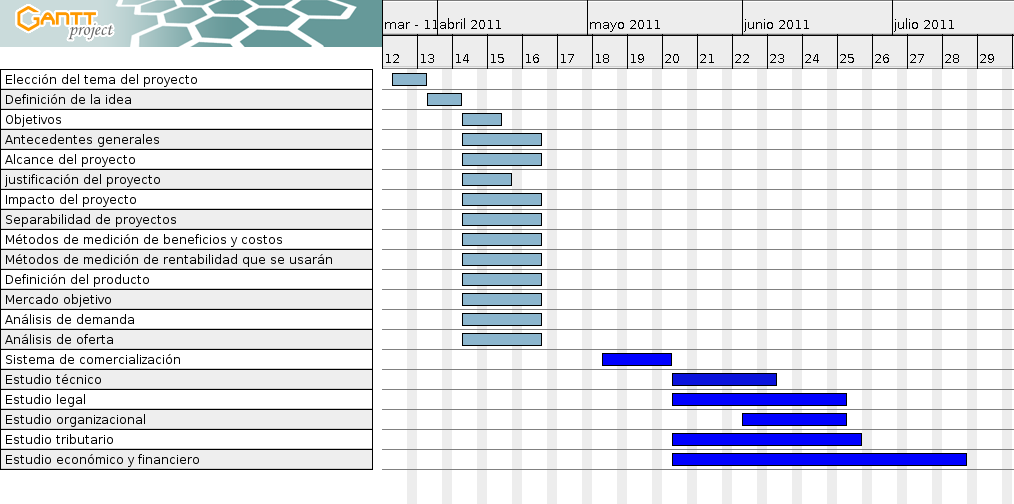
\includegraphics[scale=0.4]{img/carta_gantt.png}
\caption[Carta Gantt de las actividades de la evaluación del proyecto]{Carta Gantt de las actividades de la evaluación del proyecto}
\end{figure}
% Considerar sólo hasta fin de semestre, indicando cuando se realizará los estudios de mercado y esas cosas.
%
% Hay que definir una lista de actividades a realizar,
%

%Estudio Mercado.
%	Definición de producto. 1-2
%	Mercado objetivo. 1-3
%	Analisis de demanda.3-5
%	Analisis de oferta.3-5
%	Sistema de comercialización.4-7
%Estudio Técnico
%	Tamaño del proyecto.8
%	Localización del proyecto.8-9
%	Ingeniería del proyecto.8-13
%	Estimación y analisis de costo.12-13
%Estudio Socetario.8-9
%Estudio Legal.8-10
%Estudio Organizacional.11-13
%Estudio Tributario.8-10
%Estudio Ambiental.12-13
%Estudio Economico y financiero.14-16
%
%---------
%
%Estudio de Mercado 1-2
%Estudio Técnico 3-5
%Estudio organizacional 5-6
%Estudio legal 7-8
%Estudio ambiental 9-10
%Estudio economico 11-12
%Estudio financiero  12-14

\section{Estudio de Mercado}

\subsection{Definición del Producto}

Debido al gran aumento en  bandas emergentes que se ha notado en la V región,
surge la idea de poder integrar servicios existentes de apoyo a dichas bandas,
más nuevas ideas para ayudar al crecimiento de las bandas de la región.

\emph{Music Labs} será un servicio que reúna los elementos básicos para poder lanzar
a la fama a una banda emergente como:
\begin{itemize}
	\item Sala de ensayo
	\item Estudio de grabación
	\item Salón de eventos
	\item Asesoría personal
	\item Posicionamiento Web 2.0
\end{itemize}

Tanto el estudio de grabación como la sala de ensayo ofrecerán soporte y asesoría
técnica completa a cada banda, para poder obtener un trabajo de alta calidad.


El salón de eventos va a servir para ser la primera instancia de interacción de
las nuevas bandas con su público, ya que luego serán puestos en contacto con
distintos lugares en la zona, que son conocidos por ser la cuna para nuevas bandas.

La asesoría personal es muy similar a lo que podría ser un Mánager,
pero en este caso \emph{Music Labs} irá más allá, transformando esta figura,
en un asesor completo para las nuevas bandas,
ya que cada asesor estará respaldado por un grupo de profesionales, con experiencia en el área.

Finalmente el posicionamiento web 2.0, es una herramienta vital en el día de hoy,
debido a los grandes impactos provocados por las redes sociales.
Se ofrecerá tanto la asesoría para realizar el sitio oficial de la banda en internet,
como el posicionamiento en las distintas redes sociales, como Twitter, Facebook, MySpace, etc.

\emph{Music Labs} contará con expertos en cada área para proveer un servicio de excelencia.
Principalmente el unir estos servicios existentes (por separado),
es para poder evitar el procedimiento de buscar en distintas fuentes,
elementos que sirvan a la banda para alcanzar un solo objetivo.

Los servicios podrán ser contratados individualmente o en grupos,
ya que para \emph{Music Labs} es muy importante poder desligar de cualquier actividad que no tenga
que ver con la composición musical y el realizar música a las nuevas bandas por que muchas
de aquellas actividades quitan el tiempo a la banda, atrasando su despegue a la fama de una
manera notoria.

Los precios se fijaran de acuerdo a los valores de la competencia,
para de esta manera ofrecer la mejor oferta en el mercado.

Por otro lado se harán distintos descuentos dependiendo de la cantidad de servicios que se requiera contratar,
entre otras cosas.

Para facilitar el pago del o los servicios habrán varias modalidades de pago para adecuarse
a cada cliente en particular y se ofrecerán distintos plazos dependiendo de la cuota,
de los servicios requeridos, el numero de integrantes de la banda, los profesionales requeridos, entre otros.

En la actualidad internet es donde más se encuentra información sobre bandas emergentes,
es por esto que se hará una campaña publicitaria que constará de 3 pasos para posicionar
en la V región a \emph{Music Labs} como empresa del mercado musical. Primero se hará publicidad en las redes
sociales  para dar a conocer sin dar mayores detalles de la empresa \emph{Music Labs},
de esta forma se pretende atraer a posibles clientes curiosos por saber más sobre la empresa.

Segundo se publicará en diarios, revistas y/o cualquier medio que atraiga potenciales clientes,
dando a conocer más detalles de los servicios que se ofrecerán y/o descuentos para los primeros clientes.

Y tercero para inaugurar el lugar físico de \emph{Music Labs} se hará una fiesta (\emph{Music Labs Party})
en donde se presentará finalmente la empresa, además se invitará a personajes musicales influyentes
dentro de la V región para promocionar \emph{Music Labs}.

\emph{Music Labs} estará ubicado en el centro de la cuidad de Viña del Mar cercano a la plaza de Viña del Mar,
en donde se encontrara la oficina de asesoramiento, sala de ensayos, estudio de grabación y salón de eventos.

En primera instancia \emph{Music Labs} proveerá sus servicios dentro de la V región específicamente Valparaíso - Viña del Mar
debido a que solo en esta zona se encuentra las dependencias antes mencionada,
posteriormente se podría lanzar Musica Labs en otra región.

Sin embargo si bien \emph{Music Labs} se encuentra en Viña del Mar,
gracias a las redes sociales y el sitio Web se darán a conocer las bandas emergentes a nivel nacional
para que alcancen la fama.


\subsection{Mercado Objetivo}

El mercado musical siempre ha sido un tema de interés dentro de lo que es la población adulto-joven de Chile,
en especial dentro de la región de Valparaíso, debido a la gran afluencia de gente en la vida nocturna,
la cantidad de universidades e institutos de educación superior en la región,
dando como consecuencia un flujo creciente de gente interesada en la música.

Algo que marca lo anteriormente dicho, son los variados eventos durante el año que tienen como objetivo
difundir tanto la musica local, como de todo el país. Evento como el ``Rockodromo'', ``Rock Carnaza'',
organizados por las ``Escuelas del Rock''~\footnote{\url{http://www.escuelasderock.cl/}},
los carnavales culturales, etc, los cuales captan la atención y participación de jóvenes como
adultos.

Basándonos en los estudios del último CENSO realizado el año 2002,
se puede tener una estimación de la relación que existe entre los grupos socioeconómicos
en la V región, donde se puede notar la mayor cantidad de habitantes en la zona, por grupo.

\begin{figure}[h!]
    \centering
	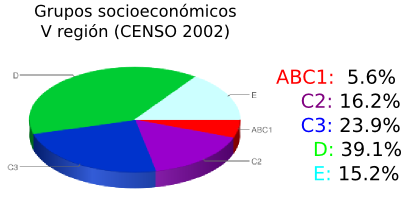
\includegraphics[width=0.6\textwidth]{img/grupos_soc}
  \caption[Porcentaje de grupos socioeconómicos de la V región]{Porcentaje de
  grupos socioeconómicos de la V región. Fuente: Instituto Nacional de
  Estadísticas de Chile.}
\end{figure}

%Es por lo anteriormente señalado, y considerando una estimación actual de la población
%en la V región, que se ha decidido realizar el presente proyecto enfocándonos en los siguientes en las personas
%mayores de 18 años, pertenecientes a los siguientes grupos socioeconómicos:


\begin{table}[h!]
\centering
\begin{tabular}{|l|l|l|}
\hline
Grupo socioeconómico & Porcentaje (\%) & Ingreso mínimo\\
\hline
C2 & 20 & 750000\\
C3 & 25 & 540000\\
\hline
\end{tabular}
\caption[Porcentaje e ingreso mínimo de grupos socioeconómico C1 y
C2]{Porcentaje e ingreso mínimo mensual por grupo familiar socioeconómico C1 y
C2. Fuente: Instituto Nacional de Estadísticas de Chile}
\end{table}

%Se descarta los grupos socioeconómicos ABC1 y D por no presentar un grupo representativo
%en las personas mayores de 18 años de la región y por no estar acorde
%a los intereses del presente producto, los que van destinados a bandas emergentes
%y sin grandes recursos. El grupo socioeconómico E se descarta por 
%no presentan ingresos necesarios para costear un servicio de este tipo.

\subsubsection{Análisis Nivel Socioeconómico C2}

\begin{table}[h!]
\centering
	\begin{tabular}{|l|p{5cm}|}
	\hline
	\textbf{Característica} & \textbf{Descripción}\\\hline
	\emph{Edad:} &	18 años o más\\\hline
	\emph{Sexo:} & 	Masculino y/o Femenino\\\hline
	\emph{Nivel socioeconómico: } & C2 / Alto \\\hline
	\emph{Educación:} & Universitario / Técnico superior\\\hline
	\emph{Ubicación:} & V Región\\\hline
	\emph{Perfil psicológico:} & Amante de la música, Creativo, viabilidad económica.\\\hline
	\end{tabular}
\caption[Descripción del público objetivo del nivel socioeconómico
C2]{Descripción de público objetivo del nivel socioeconómico C2. Fuente:
Elaboración propia.}
\end{table}

Grupo de personas con trabajo establecido, estudios universitarios profesionales
, estudios en institutos profesionales superiores, o terminando dichos estudios.
Con capacidad para costear instrumentos propios para la producción musical,
con tiempo disponible para aquello, después del trabajo o del estudio,
al estar terminándolos.

%Se considera personas del nivel C2, que poseerán cierta cantidad de recursos que puedan
%ir enfocados a un pasatiempo, como el desarrollo musical o por que no, que su
%objetivo principal sea su banda.
%
%Las personas de este nivel estarán habilitadas para poder pagar un servicio completo,
%y poder confiar en \emph{Music Labs}, para ser asesorados en todo sentido,
%dejando como única preocupación, poder madurar su banda musicalmente
%y pasarlo bien.

\subsubsection{Análisis Nivel Socioeconómico C3}

\begin{table}[h!]
\centering
	\begin{tabular}{|l|p{5cm}|}
	\hline
	\textbf{Característica:} & \textbf{Descripción}\\\hline
	\emph{Edad:} &	18 años o más\\\hline
	\emph{Sexo:} & 	Masculino y/o Femenino\\\hline
	\emph{Nivel socioeconómico: } & C3 / Medio-Alto \\\hline
	\emph{Educación:} & Secundaria / Universitario/ Técnico\\\hline
	\emph{Ubicación:} & V Región\\\hline
	\emph{Perfil psicológico:} & Creativo, amante de la música, emprendedor\\\hline
	\end{tabular}
\caption[Descripción del público objetivo del nivel socioeconómico
C3]{Descripción de público objetivo del nivel socioeconómico C3. Fuente:
Elaboración propia.}
\end{table}

Grupo de personas con estudios universitarios técnicos, estudios en institutos profesionales,
o estudios secundarios, con un trabajo estable por varios años,
con un nivel de ingresos suficiente para costear instrumentos musicales.

%Las personas del nivel C3, no poseen un sueldo lo suficientemente elevado
%para poder guardar una suma considerable y dedicarla a gastos de pasatiempos,
%por los que se piensa que el presupuesto con el que cuente una banda de nivel C3,
%no será capaz de financiar un servicio completo, sin embargo, podrá acceder
%a servicios particulares y optar a un sistema de descuentos por inscripciones,
%pues \emph{Music Labs} piensa en las dificultades económicas que puedan
%tener los posibles clientes.

\subsection{Análisis de Demanda (pasada, actual y futura)}

La búsqueda de la demanda pasada y actual está dada por diferentes factores:

\begin{itemize}
	\item Disminución de valores en instrumentos. Dada a la globalización y al aumento de la calidad de vida en Chile, se ha visto la posibilidad de importar instrumentos
de diferentes gamas, las cuales dependiendo de su calidad, va destinada a diferentes niveles de ingresos, lo que ha ayudado a que muchos se interesen en ellos 
	\item Masificación de medios de comunicación como Internet, para difusión de interés en bandas de darse a conocer. Puede que bandas se iniciaran en tiempos pasados, pero no perduraron en el tiempo y no se supo de sus existencia. Gracias a la masificación de Internet, al menos se sabe en los últimos tiempos la tendencia a iniciarse, pero sin conocer su desarrollo.
\end{itemize}

\subsubsection{Datos}

% CHILE
%A continuación se muestra en detalle la cantidad de bandas que han emergido por año en Chile, basándo tal análisis en la información dispuesta por $[1][2]$:\\
%
%\begin{center}
%\begin{tabular}{|l|l|l|l|l|l|}
%	\hline
%	año & x & y=dda & x*y & $x^2$ & $y^2$ \\
%	\hline
%	1980 & -15 & 0  & 0   & 225 & 0  \\
%	1981 & -14 & 0  & 0   & 196 & 0 \\
%	1982 & -13 & 0  & 0   & 169 & 0 \\
%	1983 & -12 & 1  & -12 & 144 & 1 \\
%	1984 & -11 & 0  & 0   & 121 & 0 \\
%	1985 & -10 & 4  & -40 & 100 & 16 \\
%	1986 & -9  & 2  & -18 & 81  & 4 \\
%	1987 & -8  & 3  & -24 & 64  & 9 \\
%	1988 & -7  & 4  & -28 & 49  & 16 \\
%	1989 & -6  & 8  & -48 & 36  & 64 \\
%	1990 & -5  & 4  & -20 & 25  & 16 \\
%	1991 & -4  & 4  & -16 & 16  & 16 \\
%	1992 & -3  & 4  & -12 & 9   & 16 \\
%	1993 & -2  & 7  & -14 & 4   & 49 \\
%	1994 & -1  & 6  & -6  & 1   & 36 \\
%	1995 & 0   & 7  & 0   & 0   & 49 \\
%	1996 & 1   & 6  & 6   & 1   & 36 \\
%	1997 & 2   & 22 & 44  & 4   & 484 \\
%	1998 & 3   & 14 & 42  & 9   & 196 \\
%	1999 & 4   & 21 & 84  & 16  & 441 \\
%	2000 & 5   & 22 & 110 & 25  & 484 \\
%	2001 & 6   & 21 & 126 & 36  & 441 \\
%	2002 & 7   & 15 & 105 & 49  & 225 \\
%	2003 & 8   & 28 & 224 & 64  & 784 \\
%	2004 & 9   & 22 & 198 & 81  & 484 \\
%	2005 & 10  & 27 & 270 & 100 & 729 \\
%	2006 & 11  & 23 & 253 & 121 & 529 \\
%	2007 & 12  & 28 & 336 & 144 & 784 \\
%	2008 & 13  & 38 & 494 & 169 & 1444 \\
%	2009 & 14  & 14 & 196 & 196 & 196 \\
%	2010 & 15  & 5  & 75  & 225 & 25 \\
%	\hline
%	$\sum$ & 0 & 360 & 2325 & 2480 & 6274\\ 
%	\hline
%	Prom & 0 & 360 & 75 & 80 & 202 \\
%	\hline
%\end{tabular}
%\end{center}

% VALPARAISO
A continuación se muestra en detalle la cantidad de bandas que han emergido por año en Valparaíso, basando tal análisis en la información dispuesta por $[1][2]$:

\begin{table}[h!]
\centering
\footnotesize
\begin{tabular}{|l|l|l|l|l|l|}
	\hline
	{\bf Año} & {\bf x} & {\bf y=dda} & {\bf x*y} & {\bf $x^2$ } & {\bf $y^2$ }\\
	\hline
	1980 &	-15	& 0	 & 0	& 225 &	0\\
	1981 &	-14	& 0	 & 0	& 196 &	0\\
	1982 &	-13	& 0	 & 0	& 169 &	0\\
	1983 &	-12	& 0	 & 0	& 144 &	0\\
	1984 &	-11	& 0	 & 0	& 121 &	0\\
	1985 &	-10	& 1	 & -10	& 100 &	1\\
	1986 &	-9	& 0	 & 0	& 81  &   0\\
	1987 &	-8	& 1	 & -8	& 64  &   1\\
	1988 &	-7	& 2	 & -14	& 49  &   4\\
	1989 &	-6	& 5	 & -30	& 36  &   25\\
	1990 &	-5	& 0	 & 0	& 25  &   0\\
	1991 &	-4	& 0	 & 0	& 16  &   0\\
	1992 &	-3	& 2	 & -6	& 9	  &   4\\
	1993 &	-2	& 0	 & 0	& 4	  &   0\\
	1994 &	-1	& 1	 & -1	& 1	  &   1\\
	1995 &	0	& 0	 & 0	& 0	  &   0\\
	1996 &	1	& 1	 & 1	& 1	  &   1\\
	1997 &	2	& 3	 & 6	& 4	  &   9\\
	1998 &	3	& 3	 & 9	& 9	  &   9\\
	1999 &	4	& 3	 & 12	& 16  &   9\\
	2000 &	5	& 4	 & 20	& 25  &   16\\
	2001 &	6	& 4	 & 24	& 36  &   16\\
	2002 &	7	& 4	 & 28	& 49  &   16\\
	2003 &	8	& 6	 & 48	& 64  &   36\\
	2004 &	9	& 3	 & 27	& 81  &   9\\
	2005 &	10	& 6	 & 60	& 100 &	36\\
	2006 &	11	& 6	 & 66	& 121 &	36\\
	2007 &	12	& 4	 & 48	& 144 &	16\\
	2008 &	13	& 4	 & 52	& 169 &	16\\
	2009 &	14	& 2	 & 28	& 196 &	4\\
	2010 &	15	& 1	 & 15	& 225 &	1\\
	\hline
	{\bf Suma}     & 0 & 67 & 390 & 2480 & 269\\
	\hline
	{\bf Promedio} & 0 & 2.1612 & 12.5806 & 80 & 8.6774\\
	\hline
\end{tabular}
\caption[Interpolación lineal de la aparición de bandas nuevas de Valparaíso]
{Interpolación lineal de la aparición de bandas nuevas de Valparaíso. Fuente:
Elaboración propia.}
\end{table}

Un hecho importante para considerar un análisis de la demanda pasada y actual de bandas, es que no se posee
una colección histórica, que indique de manera fehaciente la tendencia real se ha demostrado con el paso de los años,
por lo que el presente análisis se basa en la intención de dichas bandas en darse a conocer en medios de masificación, 
como el es Internet. Por lo explicado anteriormente, se puede apreciar que si bien en la tabla anterior se ve una demanda muy
reducida (valores entre 0 y 6 bandas), lo importante no es tanto la cantidad, sino la tendencia creciente.

\subsubsection{Demanda futura}

% CHILE
%Para obtener la tendencia de la demanda, se utiliza una regresión lineal, donde dado una cantidad $n$ de datos, el intercepto y la pendiente se detalla a continuación:\\\\
%$a = \bar{y} - b \cdot \bar{x}$\\
%$b = \frac{\sum(x\cdot y) - n \cdot \bar{x} \cdot \bar{y}}{\sum x^2 - n \cdot \bar{x}^2}$\\\\
%$b = 0.9375$\\
%$a = 360$\\
%
%Obteniendo finalmente que el comportamiento de la demanda está dado por:\\
%
%$demanda = a + bx = 360 + 0.9375x$\\

% VALPARAISO
Para obtener la tendencia de la demanda, se utiliza una regresión lineal, donde dado una cantidad $n$ de datos, el intercepto y la pendiente se detalla a continuación:

\begin{eqnarray}
a &=& \bar{y} - b \cdot \bar{x}\\
b &=& \frac{\sum(x\cdot y) - n \cdot \bar{x} \cdot \bar{y}}{\sum x^2 - n \cdot \bar{x}^2}\\
b &=& 0.15 \nonumber\\
a &=& 2.12 \nonumber\\
\end{eqnarray}

Obteniendo finalmente que el comportamiento de la demanda está dado por:\\

\begin{eqnarray}
demanda = a + bx = 2.12 + 0.15x
\end{eqnarray}

%La profesora indicó que hay que hay que obtener un \% estimativo de la demanado
%utilizando todos los medios que podamos. Éstos incluyen:
%    - Consultas de clientes de Estudios de grabación.
%    - Cantidad de grupos participantes en centros culturales y eventos
%    gratutios.
%    - Consultas a grupos existentes, etc.
%    - Servicios similares en el extranjero.

Calculo de índice $r^2$:\\

\begin{eqnarray}
r^2 = \frac{\left ( n \cdot \sum (x \cdot y) - (\sum x) \cdot (\sum y)\right )^2}{ \left (n \cdot \sum x^2 - (\sum x)^2 \right ) \cdot \left ( n \cdot \sum y^2 - (\sum y)^2 \right )}\\
r^2 = 0.4938 \nonumber
\end{eqnarray}

$r^2$ representa al coeficiente de determinación, el cual mide la proporción de
variabilidad total de nuestra demanda respecto a su media,
explicada por el modelo de regresión lineal, con lo cual podemos concluir que
la demanda posee una tendencia de crecimiento a futuro, aunque ésta tendencia
no sigue un comportamiento completamente lineal.

\begin{table}[h!]
\centering
\begin{tabular}{|l|l|l|}
	\hline
	año & x & y=dda\\
	\hline
	2011 & 16 & 4.5199\\
	\hline
	2012 & 17 & 4.6699\\
	\hline
	2013 & 18 & 4.8200\\
	\hline
	2014 & 19 & 4.9700\\
	\hline
	2015 & 20 & 5.1200\\
	\hline
\end{tabular}
\caption{Proyección de demanda}
\end{table}

Se puede apreciar que si bien se ha estimado un crecimiento mínimo, al desconocer en magnitud la demanda en forma precisa, se puede realizar una estimación
y establecer una cota inferior basado en lo anterior, que establece un crecimiento en unos 5 años, apreciable al proyectar la demanda con pendiente positiva.
% TO DO
%\red{MAYOR ANALISIS EN TABLA 5}

\subsection{Análisis de Oferta (pasada, actual y futura)}
	Los principales competidores son las salas de ensayo tradicionales, que en su mayoría sólo ofrecen el servicio de arriendo de la sala y en muy pocas ocasiones un conjunto de servicios tan completo como el propuesto en el presente proyecto.

	La siguiente tabla corresponde a una muestra de las principales salas de ensayo de la V región $[3]$: 
\begin{table}[h!]
\centering
	\begin{tabular}{|l|l|l|p{5cm}|}
	\hline
	\textbf{Empresa} & \textbf{Ubicación}  & \textbf{Valor hr.} & \textbf{Servicios}\\
	\hline
	Barcelona & Valparaíso & 3000 & Sala de ensayo\\
	\hline
	Nebadon 3.0 & Valparaíso & - & Sala de ensayo, grabación \\
	\hline
	La tocata & Villa Alemana & - & Sala de ensayo, clases de música\\
	\hline	
	Master Pro & Valparaíso & 5000 & Sala de ensayo, arriendo y venta de equipos\\
	\hline
	AFL sonido imagen & Quilpué  & 4000 & Sala de ensayo, estudio de grabación\\
	\hline
	Calaka Records & Valparaíso& 3000 & Sala de ensayo\\
	\hline	
	Estudio DIGITMIX & Viña del mar - Concon & 5000 & Sala de ensayo, estudio de grabación y arriendo de equipos\\
	\hline	
	\end{tabular}
\caption[Información de las empresas de estudios de grabación y arriendo de
salas de ensayo de la V región]
{Información de las empresas de estudios de grabación y arriendo de
salas de ensayo de la V región. Fuente: Elaboración propia.}


\end{table}

\subsubsection{Datos}

% TO DO
%\red{no corresponde a la oferta este punto}

Basándose en documentos del consejo de rectores de universidades de chile 
(CRUCH) $[4]$ actualizados al año 2009, se puede obtener la cantidad de estudiantes 
que pertenecen a universidades tradicionales de la V región. Estos datos son:

\begin{itemize}
    \item UTFSM (casa central + sede jmc): 9417 alumnos (6245 casa central, 3172 sede jmc).
    \item PUCV: 13317
    \item UV: 13120
    \item UPLA: 6464
\end{itemize}

Además, como dato obtenido desde el club de música de la UTFSM, actualmente, 
en la casa central se encuentra un total de 23 bandas compuestas por estudiantes
de esa casa de estudios. Suponiendo una relación lineal con las otras 
Universidades, se puede obtener una primera aproximación de la demanda 
(la toma de estos datos es una estimación lineal no exacta, pero sirve para 
aproximar una cantidad de potenciales clientes. Estos datos serán verificados 
con mayor exacitud dentro de los estudios siguientes). Esta primera 
aproximación corresponde a:

UTFSM, casa central: 23 bandas de un total de 6245 alumnos.
UV, 48 bandas de un total de 13120 alumnos.
PUCV. 49 bandas de un total de 13317 alumnos.
UPLA: 23 bandas de un total de 6464 alumnos.

Esto entrega un total de 143 potenciales clientes, sólo en lo referente a las 
Universidades del consejo de rectores. Por lo tanto, como primera aproximación 
en lo referente a la demanda, se puede contar con una base que corresponda 
a este número. Por otro lado, es importante notar que no se han tomado en 
cuenta Universidades Privadas ni Institutos o centros de formación técnica 
que también podrían ingresar dentro de la muestra, y que aumentarían la 
posible demanda (llegando fácilmente a las 200). 

Debido a estos datos, es importante notar que la oferta que se realice sea capaz
de abarcar la demanda.  

\textbf{Nota:} Cabe destacar que los datos aquí mencionados no fueron tomados en cuenta 
al momento de realizar el análisis de oferta inicial. Esto debido a que aún no se
cuenta con antecedentes que permitan generar una relación histórica para determinar
el crecimiento del número de bandas que se forman año a año en las universidades.
Lo mismo sucede con la figura 4, que corresponde al gráfico de la proporción de bandas
entre la V y la RM.


\subsubsection{Oferta futura}

La oferta que se debe poder lograr tiene que satisfacer la mayor cantidad
de demanda posible. Es por esto que, basados en el punto anterior, donde se
obtuvo una cantidad aproximada de bandas, se puede lograr una aproximación de 
la oferta.

Se realizó conversaciones con algunas bandas, llegando a la conclusión que
la frecuencia de ensayos es de alrededor de 4 horas semanales. Si este valor
se multiplica por la cantidad de bandas obtenidas en el punto anterior, 
se obtiene que:
\begin{center}
	\emph{Cantidad de horas totales semanales por el total de bandas}: \\
	$4\cdot 200 = 800$
\end{center} 

\emph{Music Labs} pretende crear 2 nuevas salas de ensayo, en un horario 
aproximado de atención de 9 de la mañana, hasta las 24 horas, lo que da un 
total de 15 horas disponible. Suponiendo un servicio los 7 días de la semana, 
se tendrá un total de $15\cdot7 = 105$ horas por cada sala de ensayo, dando 
un total de 210 horas en la semana, lo que abarcaría la mitad del mercado total.
Si se supone un comportamiento similar con el resto de las salas de ensayo
existentes en la región, cada una de ellas tendrá 105 horas disponibles, lo 
que da un total de 735 horas disponibles. Acá es posible darse cuenta que 
existe 65 horas que no están siendo satisfechas (notar además que no han sido
contabilizadas para este análisis las bandas que no son de jóvenes
universitarios, lo que amplia aún más esta cantidad de horas). Esto indica
que existe claramente una oportunidad de establecerse en este nicho.

La idea general de \emph{Music Labs} es poder abarcar las horas que no están siendo 
satisfechas, además de poder competir con las instalaciones que ya existen.
Para eso, se pretende realizar un crecimiento lineal anual, abarcando un 10\% extra de las horas, 
tomando como base el año anterior. Es decir, el año 1 se intentará satisfacer las 65 horas 
insatisfechas, mientras que el año 2, se tiene como meta 65 + 6.5 horas (71.5 horas). Todo esto, hasta llegar 
a la capacidad máxima del local.

%Para poder obtener una regresión lineal de la oferta, solamente teniendo un porcentaje de crecimiento, es necesario realizar un pequeño análisis geométrico.
%
%Considerando entre los años 1980 y 2010, con 1995 el punto intermedio, donde el valor de la oferta correspondería al intercepto en el eje y. Tenemos
%que la curva de regresión esta dada por:
%
%\begin{center}
%$oferta = a + bx$
%\end{center}
%
%Donde a es el intercepto y b el valor de crecimiento investigado a través de locales similares que presentarían una tendencia similar a los locales
%en los que estamos interesados.
%
%\begin{center}
%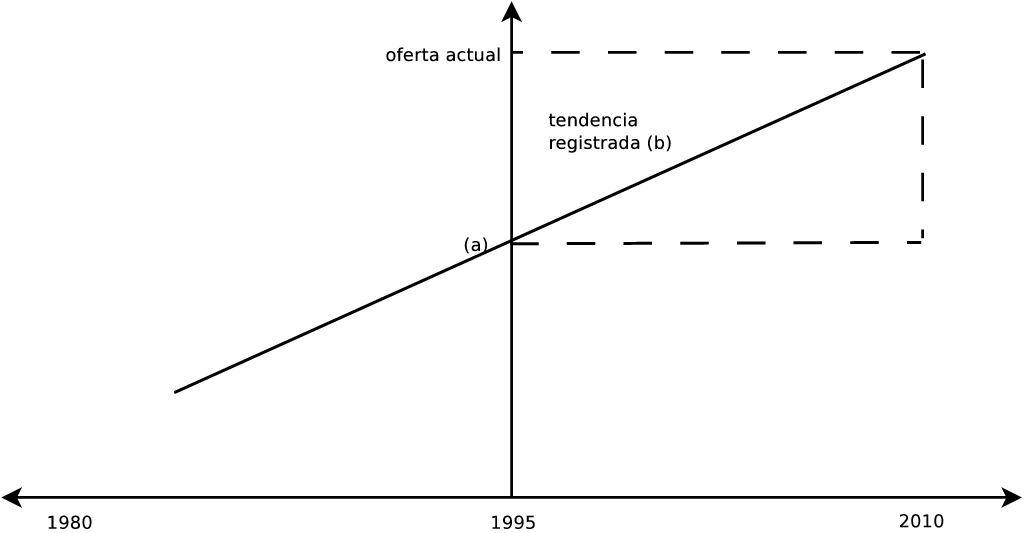
\includegraphics[scale=0.35]{img/oferta}
%\end{center}
%
%Se puede observar que mediante un calculo geométrico que:
%
%\begin{center}
%$\frac{oferta\_actual - a}{2010-1995} = b$
%\end{center}
%
%Donde b fue encontrado mediante investigación (punto anterior), por lo que es un dato conocido. Dando como resultado final para el intercepto:
%
%\begin{center}
%$a = oferta\_actual - 15b$
%\end{center}
%
%Reemplazando los valores actuales y la tendencia encontrada por investigación:
%
%\begin{center}
%a = 7 - 15b = \red{COLOCAR}\\
%b = \red{INVESTIGAR y COLOCAR, calcular lo de arriba}
%\end{center}
%
%Dando finalmente que:
%
%\begin{center}
%$oferta = a + bx$ \red{PONER CON VALORES REALES}
%\end{center}
%

\section{Bibliografías y Referencias}
\begin{enumerate}
\item Portal chileno sobre bandas emergentes. http://bandaschile.cl
\item Portal underground sobre bandas de rock chilenas.\\ http://www.infiernochileno.cl/site/index.php?p=productsList\&iCategory=3
\item Guía de Salas de Ensayo de Chile. http://www.ubik.cl/salas\_de\_ensayo.htm
\item Cuadros estadísticos por Universidad: Vacantes y Matrículas por carrera, 2009.\\ Consejo de rectores de universidades de Chile \\ http://www.cruch.cl/documentos/estadisticos2009.pdf
\end{enumerate}

\section{Anexos}
\subsection{Demanda}

\begin{figure}[h!]
    \centering
    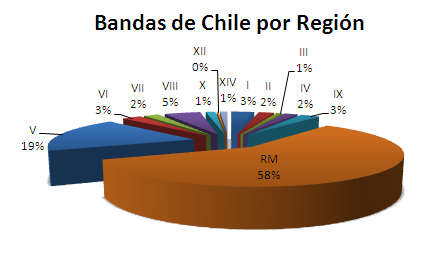
\includegraphics[scale=0.75]{img/demanda1.png}
  \caption[Proporción de bandas de Chile por regiones]{Gráfico de proporción de
  bandas por regiones. Fuente: Elaboración propia.}
\end{figure}


\begin{figure}[h!]
    \centering
    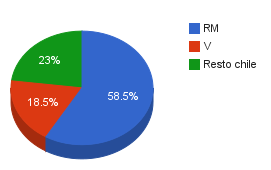
\includegraphics[]{img/demanda2.png}
  \caption[Proporción de bandas entre la V región y la RM]{Proporción de bandas
  entre la V región y la RM. Fuente: Elaboración propia.}
\end{figure}

\begin{figure}[h!]
    \centering
    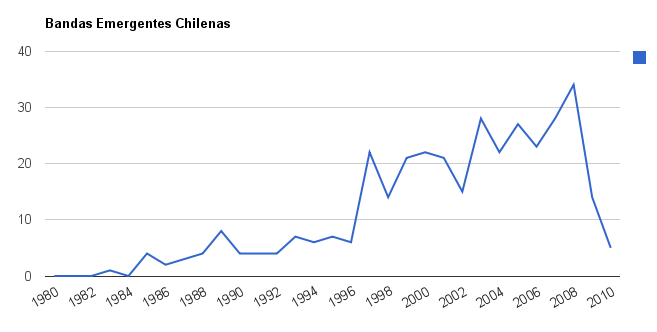
\includegraphics[angle=-90,scale=0.75]{img/demanda3.png}
  \caption[Tendencia de bandas por años en la V región]{Tendencia de bandas por
  años en la V región. Fuente: Elaboración propia.}
\end{figure}

\begin{figure}[h!]
    \centering
    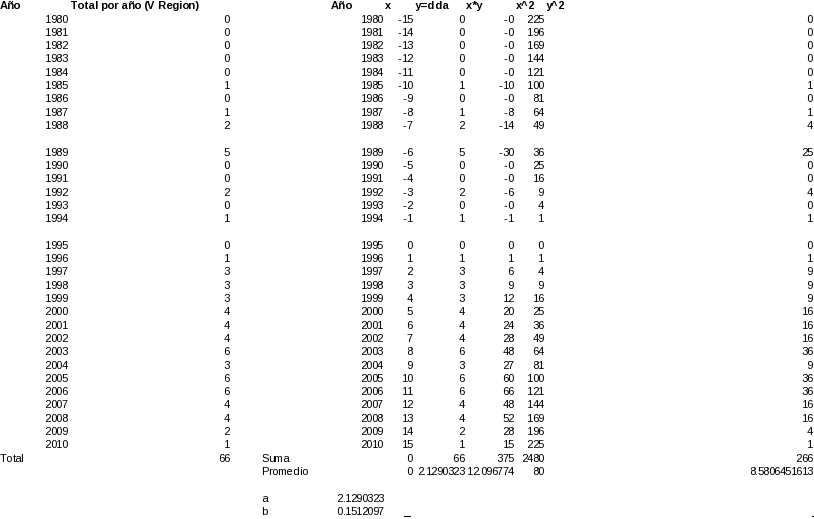
\includegraphics[scale=0.75, angle=-90]{img/demanda4.png}
  \caption[Análisis de tendencia de bandas en la V región]{Análisis de
  tendencia de bandas en la V región. Fuente: Elaboración propia.}
\end{figure}
\newpage
\subsection{Oferta}
\begin{figure}[h!]
    \centering
    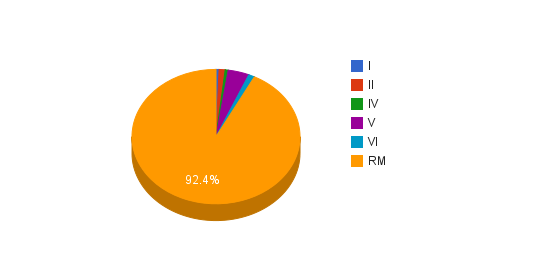
\includegraphics[]{img/oferta1.png}
  \caption[Proporción de locales de arriendo de sala y grabación por
  región]{Proporción de locales de arriendo de sala y grabación por región.
  Fuente: Elaboración propia.}
\end{figure}


%\section{Referencias}
%\bibliography{references}

\end{document}
